\section{Gestion des corrections}

\begin{center}
\scalebox{0.7}{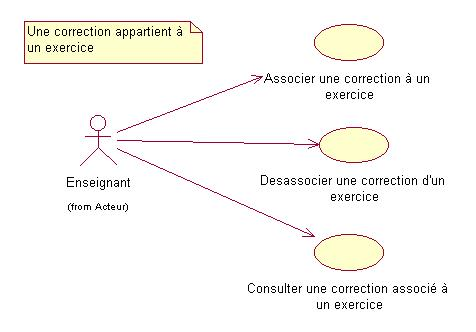
\includegraphics{images/correction.jpg}}\\
\par{Package Gestion Correction}
\end{center}

Voici les diff{\'e}rents sc{\'e}narios:\\

\section*{Enseignant}

\begin{tabular}{|p{4cm}|c|p{4cm}|p{5cm}|}
\hline
  Fonction & Priorit{\'e} & Qualit{\'e} & Mesure \\
\hline
Consulter la correction d'un exercice & 3 & Fiabilit{\'e}, Lisibilit{\'e} &
  Pas le droit de modifier la correction lors de la
  consultation. Lecture claire.\\
\hline
Associer une correction {\`a} un exercice & 3 & Fiable et Facile &
  Correction bien assign{\'e}e {\`a} l'exercice s{\'e}lectionn{\'e}. Association par
  des menus simples.\\
\hline
D{\'e}sassocier une correction {\`a} un exercice & 3 & Fiable et Facile &
  Correction bien d{\'e}sassoci{\'e} de l'exercice s{\'e}lectionn{\'e}. D{\'e}sassociation par
  des menus simples.\\
\hline
\end{tabular}

\begin{center}
{\'e}chelle de mesure de la priorit{\'e}:

\scalebox{0.5}{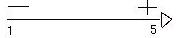
\includegraphics{images/echelle.jpg}}
\end{center}


\begin{itemize}
\item {\bf Consulter une correction {\`a} un exercice:}
	\begin{itemize}
	\item Pr{\'e}-requis : Etre log{\'e}/identifi{\'e}.\\
	L'exercice poss{\`e}de au moins une correction associ{\'e}e.
	\item Description :  L'utilisateur selectionne un exercice.\\
	L'utilisateur consulte la correction associ{\'e}e {\`a} l'exercice.
	\item Post-requis : La correction de l'exercice s{\'e}lectionn{\'e} est affich{\'e}e.
	\end{itemize}

\item {\bf Associer une correction {\`a} un exercice:}
	\begin{itemize}
	\item Pr{\'e}-requis : Etre log{\'e}
	\item Description :  L'utilisateur selectionne un exercice.\\
	L'utilisateur importe un fichier correction et l'associe {\`a} cet exercice.
	\item Post-requis : L'exercice s{\'e}lectionn{\'e} poss{\`e}de une correction associ{\'e}e.
	\end{itemize}

\item {\bf D{\'e}sassocier une correction d'un exercice:}
	\begin{itemize}
	\item Pr{\'e}-requis : Etre log{\'e}\\
	L'exercice poss{\`e}de au moins une correction associ{\'e}.
	\item Description : L'utilisateur selectionne un exercice.\\
	L'utilisateur supprime le fichier correction associ{\'e}e {\`a} cet exercice.
	\item Post-requis : L'exercice ne poss{\`e}de plus de correction associ{\'e}e.\\
	\end{itemize}
			
\end{itemize}